% Options for packages loaded elsewhere
\PassOptionsToPackage{unicode}{hyperref}
\PassOptionsToPackage{hyphens}{url}
%
\documentclass[
]{article}
\usepackage{amsmath,amssymb}
\usepackage{lmodern}
\usepackage{iftex}
\ifPDFTeX
  \usepackage[T1]{fontenc}
  \usepackage[utf8]{inputenc}
  \usepackage{textcomp} % provide euro and other symbols
\else % if luatex or xetex
  \usepackage{unicode-math}
  \defaultfontfeatures{Scale=MatchLowercase}
  \defaultfontfeatures[\rmfamily]{Ligatures=TeX,Scale=1}
\fi
% Use upquote if available, for straight quotes in verbatim environments
\IfFileExists{upquote.sty}{\usepackage{upquote}}{}
\IfFileExists{microtype.sty}{% use microtype if available
  \usepackage[]{microtype}
  \UseMicrotypeSet[protrusion]{basicmath} % disable protrusion for tt fonts
}{}
\makeatletter
\@ifundefined{KOMAClassName}{% if non-KOMA class
  \IfFileExists{parskip.sty}{%
    \usepackage{parskip}
  }{% else
    \setlength{\parindent}{0pt}
    \setlength{\parskip}{6pt plus 2pt minus 1pt}}
}{% if KOMA class
  \KOMAoptions{parskip=half}}
\makeatother
\usepackage{xcolor}
\IfFileExists{xurl.sty}{\usepackage{xurl}}{} % add URL line breaks if available
\IfFileExists{bookmark.sty}{\usepackage{bookmark}}{\usepackage{hyperref}}
\hypersetup{
  pdfauthor={NPFC Bottom Fisheries Small Working Group},
  hidelinks,
  pdfcreator={LaTeX via pandoc}}
\urlstyle{same} % disable monospaced font for URLs
\usepackage[margin=1in]{geometry}
\usepackage{graphicx}
\makeatletter
\def\maxwidth{\ifdim\Gin@nat@width>\linewidth\linewidth\else\Gin@nat@width\fi}
\def\maxheight{\ifdim\Gin@nat@height>\textheight\textheight\else\Gin@nat@height\fi}
\makeatother
% Scale images if necessary, so that they will not overflow the page
% margins by default, and it is still possible to overwrite the defaults
% using explicit options in \includegraphics[width, height, ...]{}
\setkeys{Gin}{width=\maxwidth,height=\maxheight,keepaspectratio}
% Set default figure placement to htbp
\makeatletter
\def\fps@figure{htbp}
\makeatother
\setlength{\emergencystretch}{3em} % prevent overfull lines
\providecommand{\tightlist}{%
  \setlength{\itemsep}{0pt}\setlength{\parskip}{0pt}}
\setcounter{secnumdepth}{-\maxdimen} % remove section numbering
\usepackage{booktabs}
\usepackage{longtable}
\usepackage{array}
\usepackage{multirow}
\usepackage{wrapfig}
\usepackage{float}
\usepackage{colortbl}
\usepackage{pdflscape}
\usepackage{tabu}
\usepackage{threeparttable}
\usepackage{threeparttablex}
\usepackage[normalem]{ulem}
\usepackage{makecell}
\usepackage{xcolor}
\ifLuaTeX
  \usepackage{selnolig}  % disable illegal ligatures
\fi

\title{Species Summary\\
North Pacific Armorhead}
\author{\emph{NPFC Bottom Fisheries Small Working Group}}
\date{\emph{2021-07-15}}

\begin{document}
\maketitle

\hypertarget{splendid-alfonsino-beryx-splendens}{%
\section{\texorpdfstring{Splendid Alfonsino (\emph{Beryx
splendens})}{Splendid Alfonsino (Beryx splendens)}}\label{splendid-alfonsino-beryx-splendens}}

\textbf{Common names:} Splendid Alfonsino (English); 红眼金鲷 (Chinese);
キンメダイ (Japanese); 빛금눈돔 (Korean); Низкотелый берикс (Russian)

\hypertarget{biological-information}{%
\subsection{Biological Information}\label{biological-information}}

Global distribution ranges from tropical to temperate oceans. Historical
catch records in the Emperor Seamount suggest the distribution from
Nintoku (45 °N) to Hancock (30 °N). Settlement occurs following a
certain period of the pelagic life stage. Adults show a vertical
distribution from 200 to 800 m with diel vertical migration, feeding on
crustaceans, cephalopods, and fish during the night. Limited information
is available for recruitment and reproduction processes in the Emperor
Seamounts, whereas the population in the Japanese coast shows 4--5 years
to sexually mature and spawning occurs during summer.

\begin{figure}

{\centering 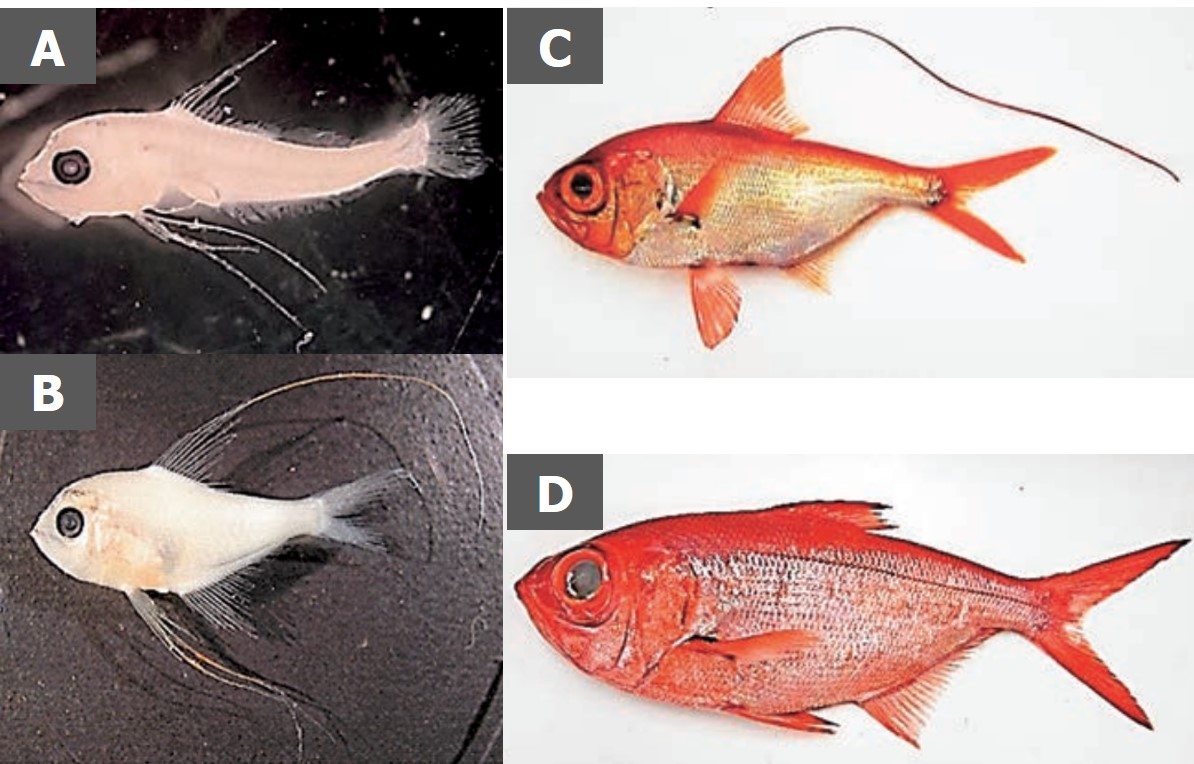
\includegraphics[width=0.7\linewidth,height=0.7\textheight]{Figures/SA} 

}

\caption{**Figure 1: Photographs of Beryx splendens.** <br>A) postlarva, B) juvenile, C) young, D) adult (from Watari et al. 2016)</br>}\label{fig:picture}
\end{figure}

\begin{figure}

{\centering 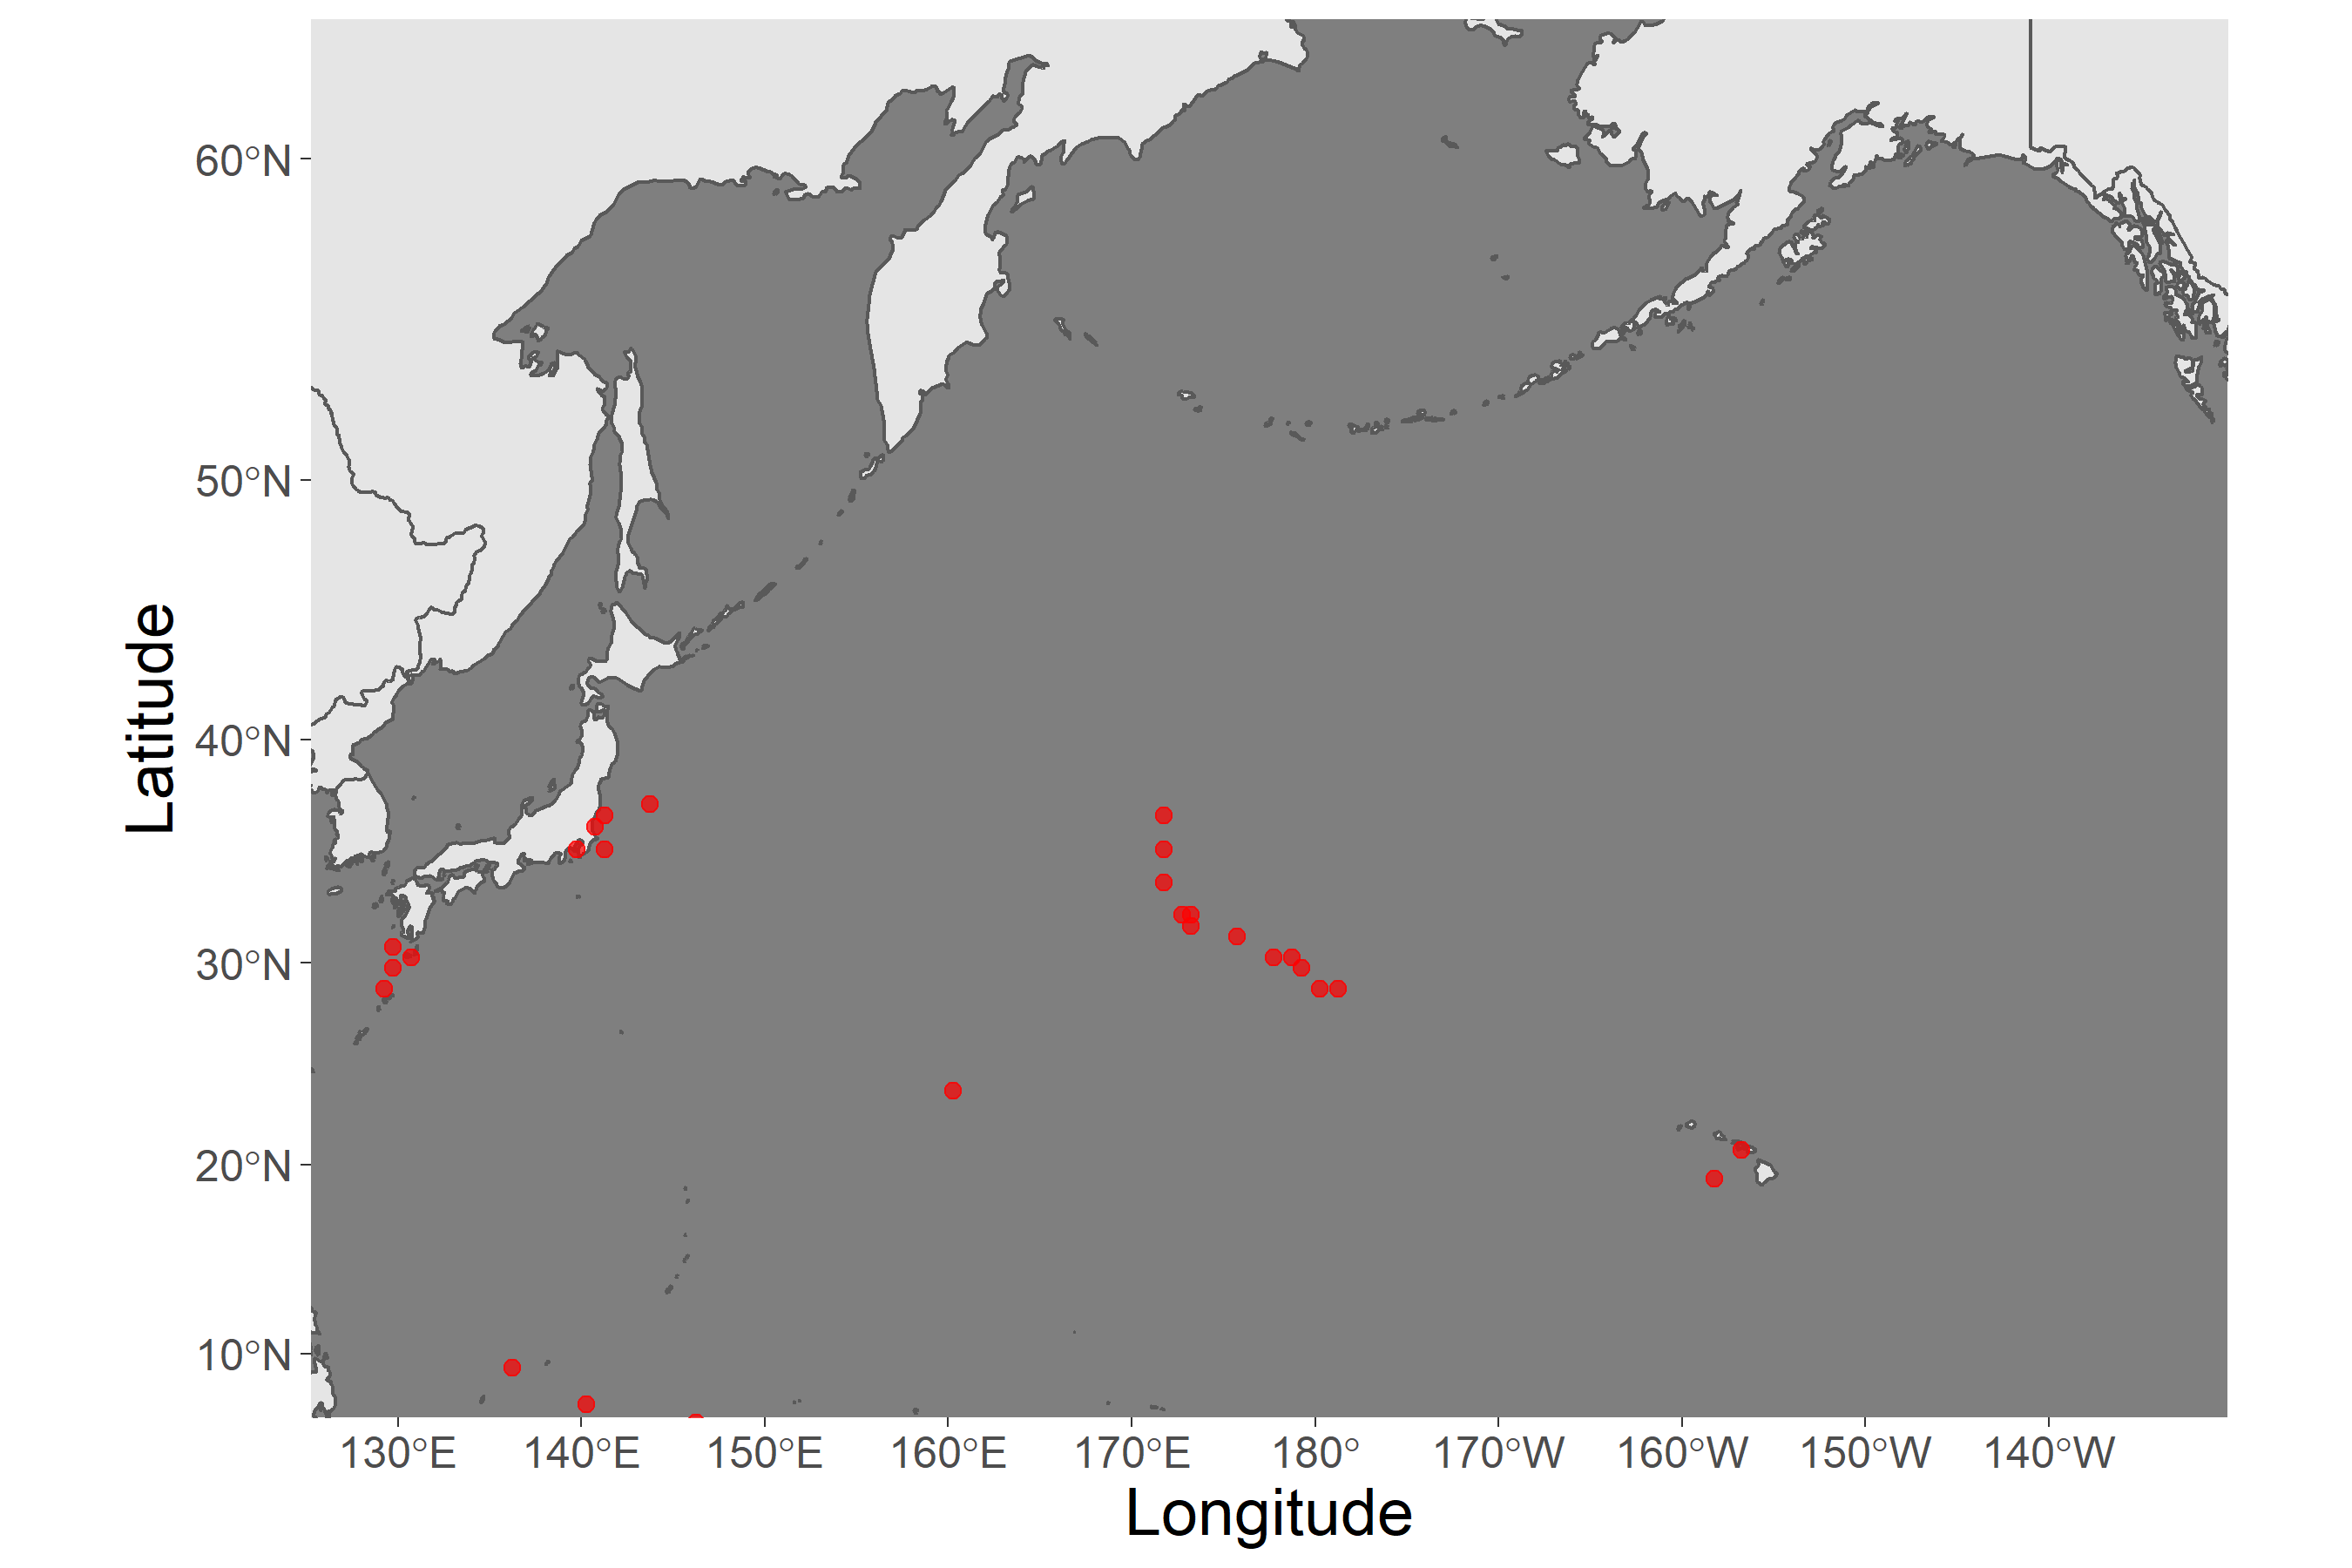
\includegraphics[width=0.8\linewidth,height=0.8\textheight]{Figures/SA_DistributionMap} 

}

\caption{**Figure 2: Known distribution of Beryx splendens.** <br>Points indicate observation data from original sources (AquaMaps 2019, October)</br>}\label{fig:picture2}
\end{figure}

\hypertarget{fishery}{%
\subsection{Fishery}\label{fishery}}

Since the discovery of large populations of North Pacific Armorhead
(NPA) in the Emperor Seamount in the late 1960s, SA has been exploited
as an alternative resource to NPA due to the large temporal fluctuation
of the NPA population. The main fishing methods are bottom trawls and
gillnets.

Historical catch record (Figure 3) shows the highest catch proportion by
Japan, followed by Korea and Russia. Russia terminated their fishery
nearly a decade ago. Fishing pressure somewhat reflects the recruitment
condition of NPA. In 2010 and 2012, when high recruitment of NPA
occurred, the annual catch decreased below 1,000 tons, whereas it
increased up to 4,000 tons ever since then.

Size composition analysis from the catch data by Japanese trawlers
suggests the substantial decrease in size of fish in catches over the
past decade, raising the concern about recruitment overfishing.

\begin{figure}

{\centering 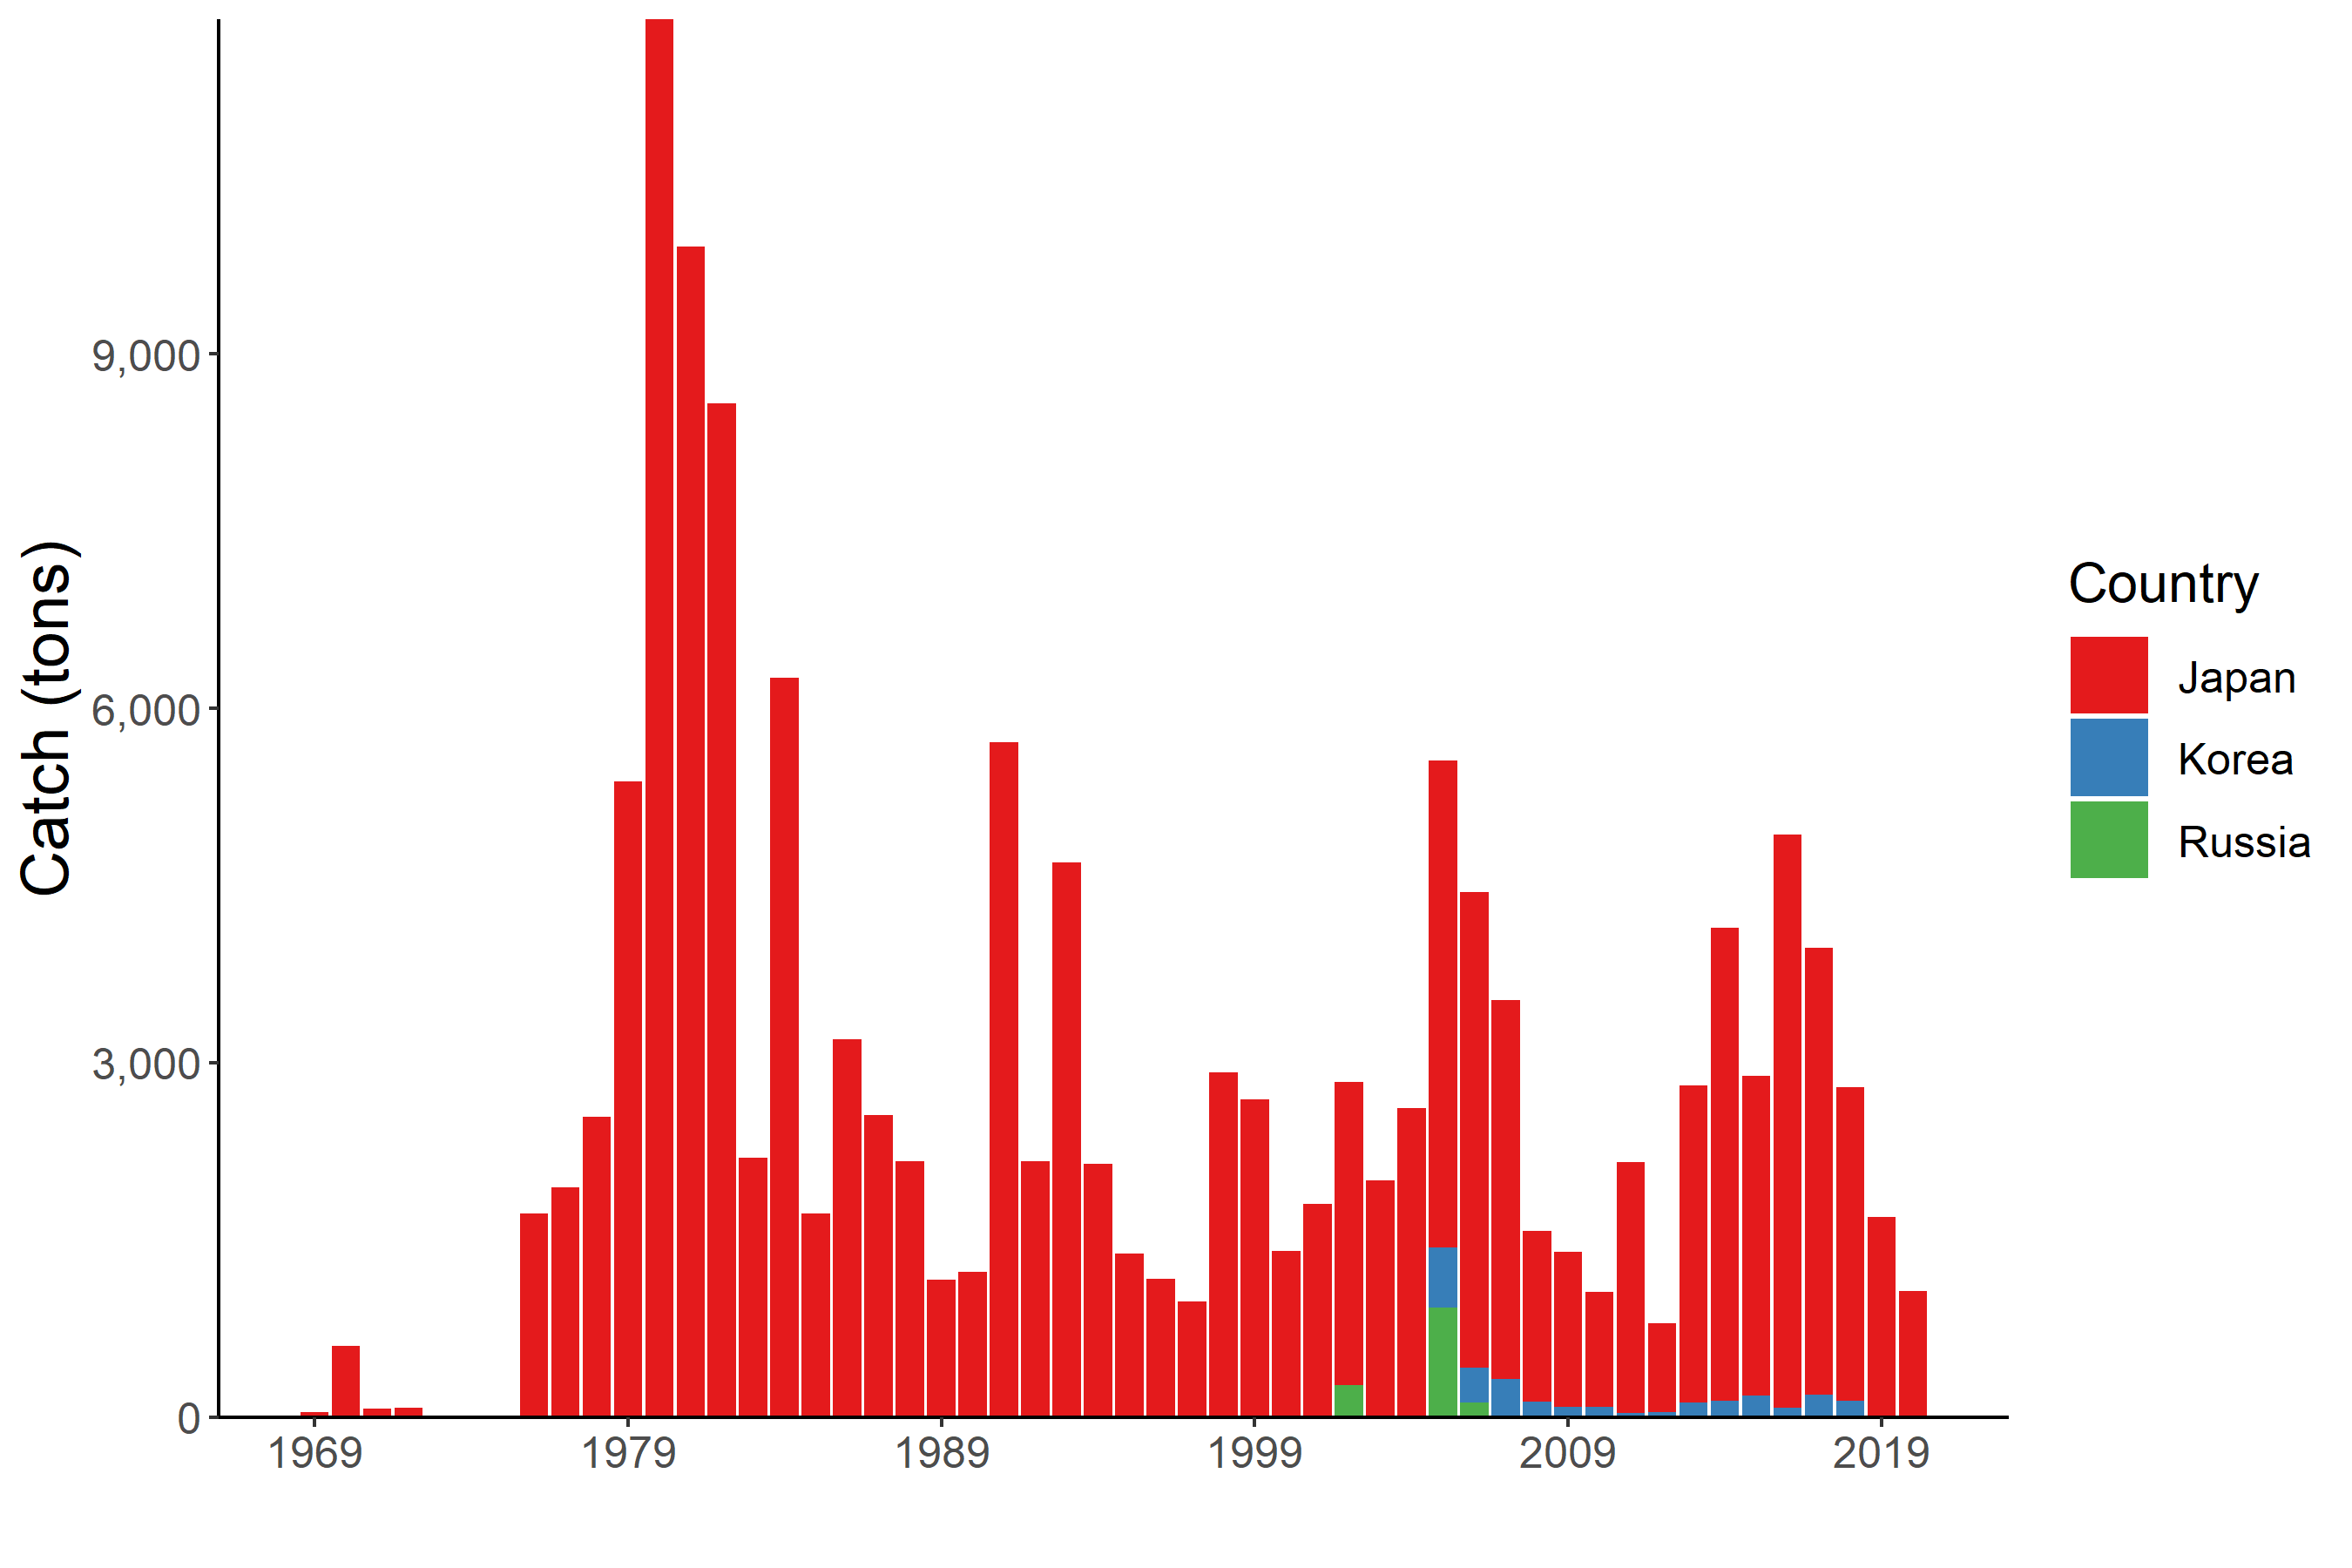
\includegraphics[width=0.8\linewidth,height=0.8\textheight]{Figures/SA_Catch} 

}

\caption{**Figure 3: Catch trends of splendid alfonsino over the past two decades.** The annual amounts of catch for alfonsino by each Member are shown by the bar plot.}\label{fig:picture3}
\end{figure}

\begin{figure}

{\centering 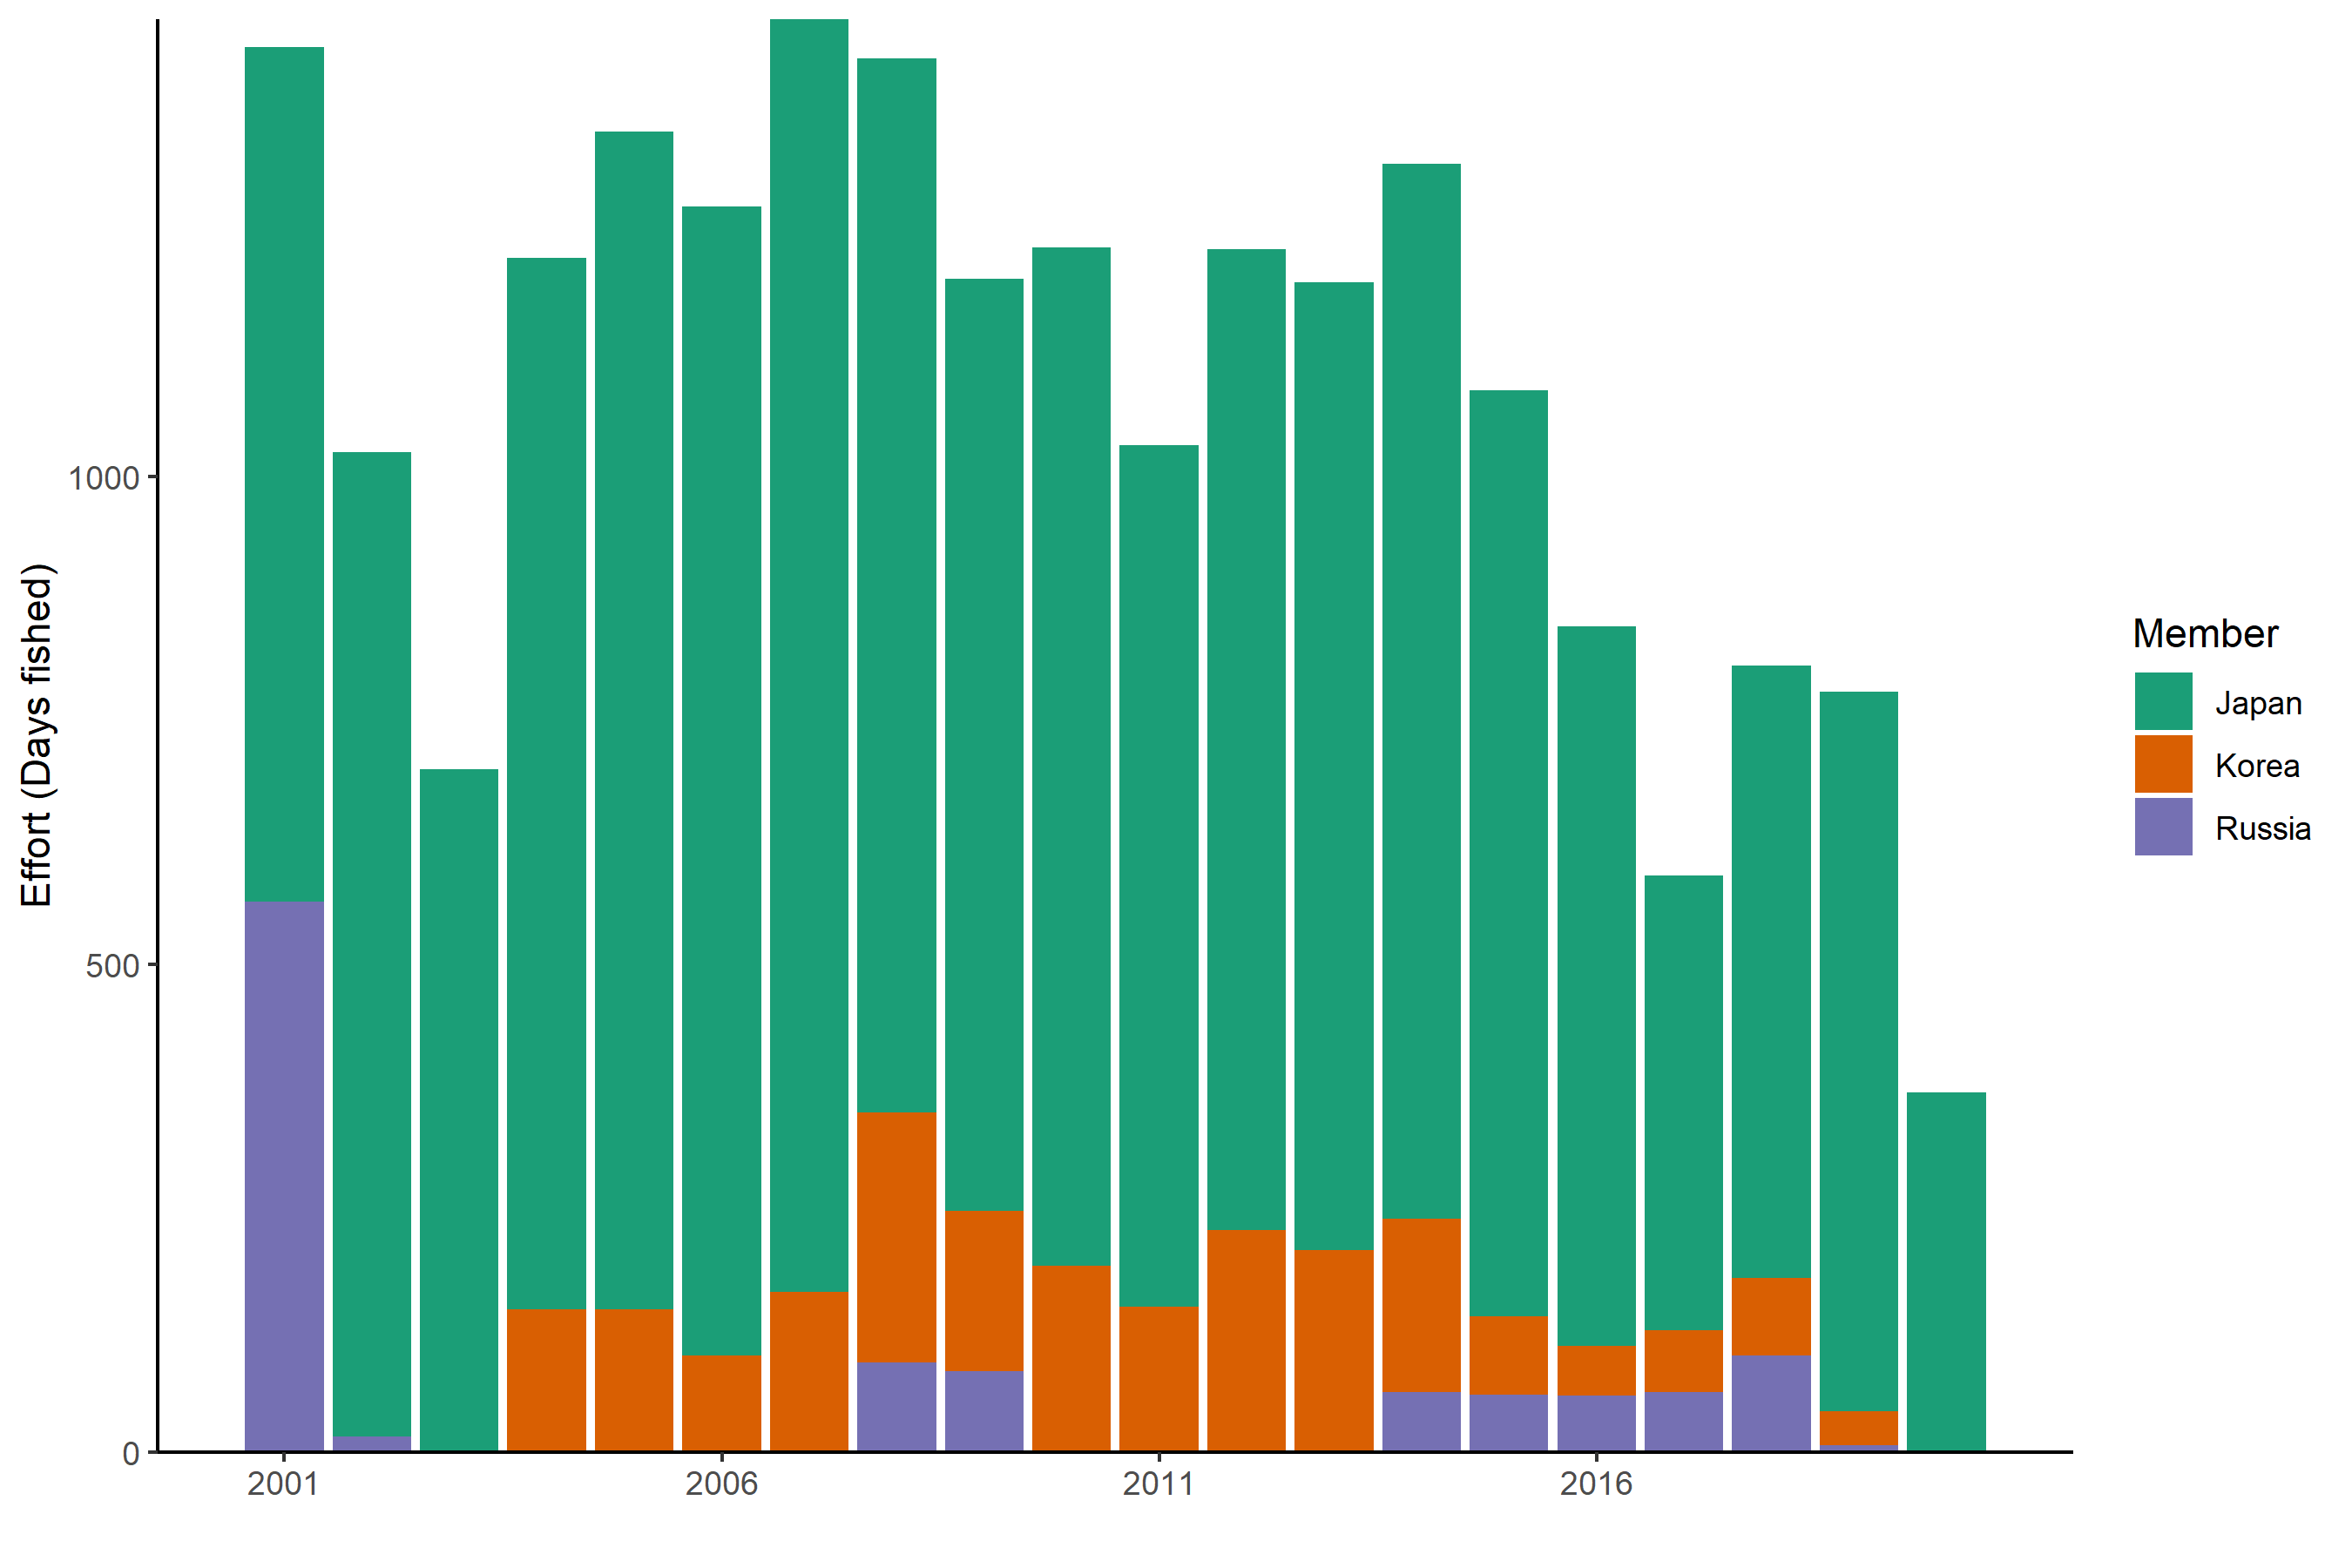
\includegraphics[width=0.7\linewidth,height=0.7\textheight]{Figures/SA_Effort} 

}

\caption{**Figure 4. Historical fishing effort for Splendid Alfonsino.**}\label{fig:picture1}
\end{figure}

\hypertarget{assessment}{%
\subsection{Assessment}\label{assessment}}

There are no biomass estimates available for SA in NPFC waters.

An age- or length-structured stock assessment may be feasible given the
life history SA (citation for more information). Surplus production
models developed by Japan in 2008 showed that the average fishing
mortality is 20--28 \% higher than the MSY level. This analysis,
however, remains unreliable as the estimated CPUE is biased due to
target shifts between NPA and SA and the estimated intrinsic population
growth rate parameter was too high for long-lived deep-sea fish.

Data limited approaches, such as YPR or SPR analysis that do not require
detailed resource parameters or fishing data, should be explored in the
future.

\hypertarget{management}{%
\subsection{Management}\label{management}}

\textbf{Active Management Measures}

The following NPFMC conservation and management measures pertain to this
species:

\begin{itemize}
\item
  CMM 2019-05 For Bottom Fisheries and Protection of VMEs in the NW
  Pacific Ocean
\item
  CMM 2019-06 For Bottom Fisheries and Protection of VMEs in the NE
  Pacific Ocean
\end{itemize}

Available from
\url{https://www.npfc.int/active-conservation-and-management-measures}

Currently, there is no accepted harvest control for this species.

In 2016, the interim management measures were implemented, which
includes limiting the fishing effort to the 2007's catch level,
prohibiting fisheries from November to December (which corresponds to
the spawning season for NPA) and not allowing fisheries in C-H Seamount
and the southeastern part of Koko Seamount (for the protection of VMEs).

In 2019, an adaptive management plan was additionally adopted, which
includes the regulation of the mesh size (trawl: \textgreater{} 10 cm,
gillnet: 12 cm) to protect juvenile fish. Still, this measure is
insufficient as the substantial catch of young fish has been reported by
trawlers even after being implemented.

\hypertarget{data-summary}{%
\subsection{Data Summary}\label{data-summary}}

\hypertarget{references}{%
\subsection{References}\label{references}}

AquaMaps 2019, October (add citation for map here)

FAO. (2016). Global review of Alfonsino (Beryx spp.) their fisheries,
biology, and management. In \emph{Food and Agriculture Organization of
the United Nations} (Vol. 1084, Issue 1084).
\url{http://www.fao.org/3/a-i5336e.pdf}

Sawada, K., Nishida, K., Yonezaki, S., Kiyota, M., \& Review, M. (2018).
\emph{Review of biology and fisheries of splendid alfonsino Beryx
splendens , especially in the Emperor seamounts area by April 2018 This
paper may be cited in the following manner: NPFC-2018-SSC BF01-WP03
Review of biology and fisheries of splendid alfonsino}.

Watari et al.~2016 (add citation information here)

\end{document}
